\chapter{A Simulation-based Exploration of Capacity}
\label{cha:capacity}
In the previous chapter, we presented a simple model for energy capacity and explored the effect of capacity on the amount of energy captured by a system. 
We utilized synthesized energy harvesting traces from an existing irradiance trace dataset, however we simplified the analysis by assuming a static average workload power.
This chapter will explore expanding our model to utilize several different dynamic workloads based off of benchmarks of real hardware, as well as considering a wireless sensor state machine that better captures the behavior of a real sensor.
The rest of the chapter is an analysis of the performance of these simulated wireless sensor workloads under real harvesting conditions.

\section{Upgrading Our Model}
\label{sec:capacity:modelling}
%The model and analysis we presented in \cref{sec:intuition:capacity} does not consider
%workload variability, and simplifies workload to an average.
In \cref{sec:intuition:capacity}, we argued that a sensor workload, which is often periodic or event driven, does not vary significantly beyond a few hours to a day of operation when compared to the variability of energy harvesting income. Photovoltaic harvesting can vary significantly over the course of a day and throughout a year. 
To verify this assumption and expand our analysis of capacity, we seek to to explore the dynamic effects that energy
capacity and backup storage have on sensor performance in the face of workload variability.
We use representative energy harvesting traces, measurements of real hardware,
and synthesized dynamic workloads in a new model based on a simple wireless sensor state machine.
We use this model to simulate
the behavior of energy harvesting sensors. 
From the input traces of workload and energy harvesting income, our model produces estimates of sensor energy utilization, availability, responsiveness, and lifetime.

\placefigure{tab:capacity:rep}

\subsection{Energy Harvesting Income}
As in \cref{sec:intuition:capacity}, we utilize the EnHANTs irradiance trace dataset as energy income for our simulation.
Unlike our previous analysis, we do not use synthesized traces, and instead utilize the traces directly.
We choose to narrow our focus to two of the traces that we think most accurately represent indoor lighting conditions: Setup A and Setup D.
As shown in \cref{fig:intuition:traces}, Setup A represents a location that receives some sunlight but is mostly lit by artificial sources while Setup D represents a location near a window that receives significant light during part of the year.
Beyond \cref{fig:intuition:traces}, these traces are summarized in \cref{tab:capacity:rep}.
On average, Setup A provides an average of 15.1\ssi[per-mode=symbol]{\micro\watt\per\centi\meter\squared} which is on the lower end of expected irradiance in indoor environments. Setup D represents the higher end of indoor irradiance with an average 97.4\ssi[per-mode=symbol]{\micro\watt\per\centi\meter\squared}.

\subsection{Representative Hardware}
We limit our analysis to the effects of capacity,
independent of the differences of energy intensity or efficiency in device
component selection. To do so, we define an example photovoltaic energy harvesting
sensor platform that utilizes currently available commercial
components.
We choose new
components in an attempt to better represent prior energy storage designs and
give them the benefit of the improvements that have occurred in recent years.
We take benchmark
measurements of various tasks performed by this platform, such as the
amount of time and energy required to sample a sensor or send a Bluetooth Low
Energy (BLE) packet. These benchmarks are used to generate energy utilization metrics
for our representative workloads shown in \cref{tab:capacity:rep}.
The physical size of the solar panel used by this sensor
is assumed to be
10.9~cm\textsuperscript{2} and the volume of the sensor node is similar to prior
work like the Hamilton sensor~\cite{kim2018system}.
%We implement this design and describe it further in \cref{sec:impl:permamote}.

\subsection{Representative Workloads}
We find that sensing workloads generally fall into three
categories: (i) periodic sense-and-send~\cite{mainwaring2002wireless}, (ii) reactive event detection~\cite{campbellEnergy14,afanasov2020battery}, and (iii) infrequent,
long-running, high-energy events~\cite{levis2004trickle}. We choose a representative workload for each
of these categories to use in our model.
We characterize our ``periodic sense-and-send''
workload as periodically sampling a light and color sensor and sending a
BLE
advertisement containing the data.
Our ``reactive workload'' is
represented by sending a BLE advertisement upon motion detection of the main
entrance of a university building, and we linearly scale the frequency
of these events to create synthetic traces with varying amounts of usage. 
We treat these workloads as atomic. 
When a packet is sent in response to a periodic schedule or a detected event, the energy spent on sending that packet must be spent instantaneously and atomically.  
Finally, our ``infrequent expensive'' workload is a
contiguous
task that is representative of an
over-the-air firmware update, which is randomly executed with an average occurrence rate
of once every two weeks.
We optimistically assume these long running tasks can be interrupted
and resumed at any point during execution and that any checkpointing does not incur any overhead.

\placefigure[t]{tab:parameters}

\section{An Energy Model for Wireless Sensors}
We use the previously discussed indoor irradiance traces, generalized
workloads, and hardware characterizations to model the behavior of sensors
using different types and sizes of energy storage. We develop an open
source\footnote{\url{https://github.com/lab11/permamote/tree/master/simulator}}
iterative simulator that allows parameterization of various system
characteristics, including regulator efficiency, solar harvester size
and efficiency, energy storage capacity, leakage, ESR, and charge-discharge
efficiency. These parameters are summarized in \cref{tab:parameters}.

The simulation of our model operates as a second-by-second calculation of the
amount of energy entering and exiting a device, similar to the model presented in \cref{sec:intuition:capacity}.
At every step, the simulation calculates the net energy gain or loss of the
system based on its current state and available stored energy.  Occasionally,
the model performs a workload event based on either a periodic schedule (in the
case of a sense-and-send workload) or from a random distribution (reactive
event detection or a high-energy event). For our modeling, workload schedules
are generated from values listed in \cref{tab:capacity:rep}.
This simulation is performed for the entirety of an
input irradiance trace, which constitutes about a year of data. During
a simulation, metrics such as energy utilization, the fraction of completed
events versus expected events, and events' time to completion are collected,
and if applicable, the primary-cell lifetime is estimated from a trace of its capacity over time.

\placefigure{fig:capacity:statemachine}

During simulation, modeled devices can be online or offline and idle or performing
work. These states are shown in \cref{fig:capacity:statemachine}.  A device's state
transitions from top to bottom of this figure and vice versa depending on the
energy state of the secondary storage.
If the secondary-cell energy state drops below \texttt{min\_hyst},
the state of the system moves to the upper
half (\textsf{offline}) of this diagram. The state of the system moves downward (\textsf{online})
if the state of charge of the secondary reaches the \texttt{max\_hyst}
limit. 
Secondary charging hysteresis limits are defined by parameters described in \cref{tab:parameters}.
A device's state can also move
to the right or left of the state machine depending on whether a workload event
is scheduled, or the prescribed workload has been completed. A new
workload event is counted as failed if the device is not in the \textsf{Online
Idle} state when it begins.
In the case of the ``atomic''
sense-and-send and reactive workloads, the modeled device will only begin
to perform an expected workload event if it has
enough energy to perform the event in entirety. If the workload is not atomic,
the device will only begin scheduled work if it has enough energy to make the
configured minimum amount of progress. We
make an assumption that the duration of atomic events are less than the one
second simulation step.
We also assume that a modeled sensor has perfect, zero-energy progress
latching and can go to sleep at any point after an active event. 
If there is energy remaining after performing a task, the modeled sensor will
attempt to spend the rest of the simulation period in the \textsf{Online Idle} state.

If the simulated device is configured with a backup primary-cell, offline
states transform to "primary" states in which the device remains on and
able to perform work, but charges energy usage to the primary storage instead
of the secondary. During these periods, the secondary cell continues charging
from harvested energy. Upon reaching the upper charging hysteresis
limit, the device returns to an online state, using energy stored in the
secondary.  If the primary storage is depleted, the simulation ends early.

\placefigure{fig:usage}

\section{Capacity Increases Energy Capture}
\label{sec:capacity:capture}

In addition to relaxing the need for intermittent techniques, we find that
an increase in sensor energy capacity
achieves a significant return on sensor
reliability and capability in the face of variable energy income.  Higher
energy capacity allows higher energy capture during periods of abundant
harvestable energy.

\subsection{Ambient Energy Utilization}
\label{sec:capacity:utilization}

Ambient energy is underutilized when it is not used to support the specified
sensing application. This may happen for two reasons: 1) 
the secondary
energy storage is full but energy is still available for harvesting, and 2) the
sensor performs work based on its energy state rather than its application
goals. The first scenario is common for energy harvesting systems
presented in prior work that charge up a capacitor and wait for an event
before sensing and sending, failing to capture all energy that may
have been harvested while their capacitor was full~\cite{campbellEnergy14, afanasov2020battery}.
For an example of the second scenario, consider
systems that transmit a packet every time their energy storage capacitor
is full rather than saving this energy for use during periods of lower harvesting
potential~\cite{hesterFlicker17, colinReconfigurable18}. Another example of this are sensors in which the harvesting
rate is proportional to the sensed phenomena~\cite{debruin2013monjolo}.
While compelling for their simplicity, these sensors use
energy that could alternatively be saved and used
later for event detection or tasks like data summarising or analysis.

To explore ambient energy utilization as a function of storage size, we
model the charge-discharge patterns of idealized energy stores under
the harvesting conditions and workloads described in \cref{sec:capacity:modelling}.
This modeling is primarily accounting for our first classification of
wasted energy, since our workload definitions \textit{do not} perform
tasks in response to available energy; instead they attempt to maximize the success
rates for the specified sensing tasks.
The results of this modeling are shown in \cref{fig:usage}. No matter
the amount of available energy, utilization increases as
storage capacity increases. For scenarios with low harvesting potential and high
power workloads, a sensor with at least 1\ssi{\milli\Wh} of storage can accomplish 100\% utilization.
In cases of
high harvesting potential and low power workloads, utilization often
stops increasing before reaching 100\%. This
can be attributed to a small fraction of the available energy being sufficient
to fully support the sensing task.
Small increases in utilization
have significant impact on reliability and system lifetime.
\placefigure{fig:reliability}

\subsection{Application Reliability}
\label{sec:store:reliability}

We also model the ability of varying energy stores to meet our defined
sensing tasks and intensities. Our results are
shown in \cref{fig:reliability}. 
Similar to the results of \cref{sec:store:utilization}, we see marked
increases in performance when energy stores reach 1-10\,mWh
of capacity.
Simulations experience 100\% reliability for all but
the most energy constrained scenarios with high power workloads and
$\geq$2\,mWh of energy storage.
We also see that even when low capacity sensors
have large energy harvesting potentials and infrequent workloads, they experience low
reliability.
This is because they
do not have enough storage to keep sensing throughout the night.

Finally, we analyze the ability of different storage configurations to perform a
random, contiguous, higher energy task. We use a 100\,mJ (30\,\textmu Wh) event that is representative of a
50\,KB over-the-air code update. While this is larger than a code update would be
for simple programs,
we see in \cref{fig:reliability:otattc} that nearly all of the configurations with
0.28\,mWh of energy storage complete the task in the minimum time (5\,s). In comparison,
even reducing the amount of energy storage to match the amount of energy
required for the code updates causes significant latency. It is clear that
many of the updates for smaller energy storage configurations
do not complete for 1000-10,000\,s.
This aligns with the amount of time a sensor may sit
idle overnight waiting for solar power.

% Mayfly/Flicker
% - Timekeeper: 1 10uF 0805YD106KAT2A 0.09 @ 100 (equiv 0.03 @ 100) (0.023)
% - MCU: 1 22uF Not specified, but an AVX 1210 costs 0.44 @ 100 (equiv 0.079 @ 100) (0.025)
% - Acel 1 2.2uF EMK107BJ225KA-T 0.039 @ 100 (equiv 0.036 @ 100) (0.015)
% - BLE  1 47uF GRM31CR60J476ME 0.21 @ 100 (equiv 0.16 @ 100) (0.028)
% - HUM  1 15uF C2012X7S1A156M125AC 0.37 @ 100 (equiv 0.19 @ 100) (0.052)
% - Press 1 33uF C3216X5R0J336M130AC 0.44 @ 100 (equiv 0.38 @ 100) (0.034)
%
% Capybara
% - test 1: 400uF ceramic (4x100 0.31 equive @100) (0.043), 330uF tant (0.69 equiv @100) (0.24), 67.5 mF super (?? $21?, $2.42)
% - test 2: 300uF ceramic (3x100), 1100uF tant ($2.43) (0.62), 7.5 mF super ($2.42) (
% - test 3: 300uF cerami (3x100)c, 100uF tant ($0.28) (0.17), 7.5 mF super ($2.42)
%
% Gecko Power Supply
% - 5 TLJG227M004R3000 1.39 @ 100 (0.37 equiv, 0.16 ali)
%
% Wisp
% - 1 10uF ?? $0.05 @ 100
\begin{definefigure*}{fig:primary}
  \centering
  \begin{subfigure}{0.39\textwidth}
    \centering
    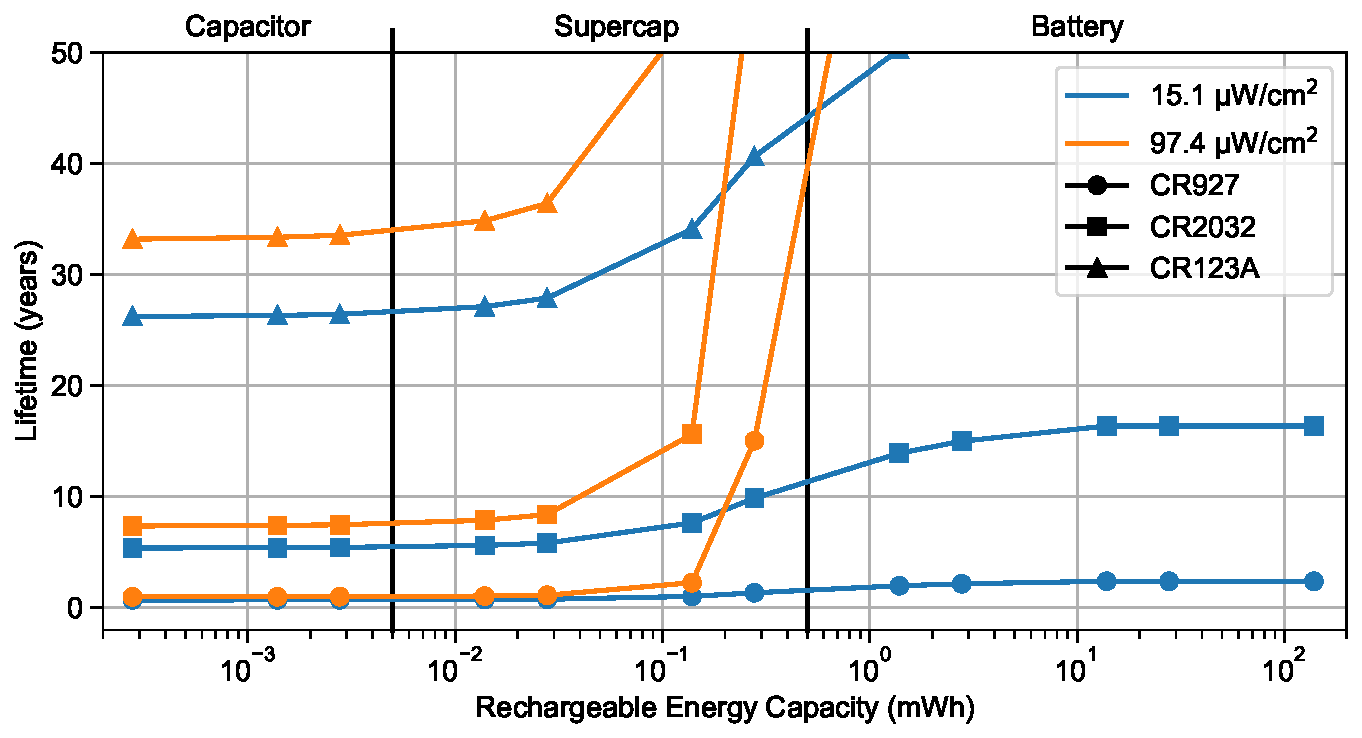
\includegraphics[width=0.85\linewidth]{figs/capacity/primary/sense_and_send_life_vs_sec_size}
    \caption{Periodic Application}
    \label{fig:primary:sensesec}
  \end{subfigure}
  \begin{subfigure}{0.6\textwidth}
    \centering
    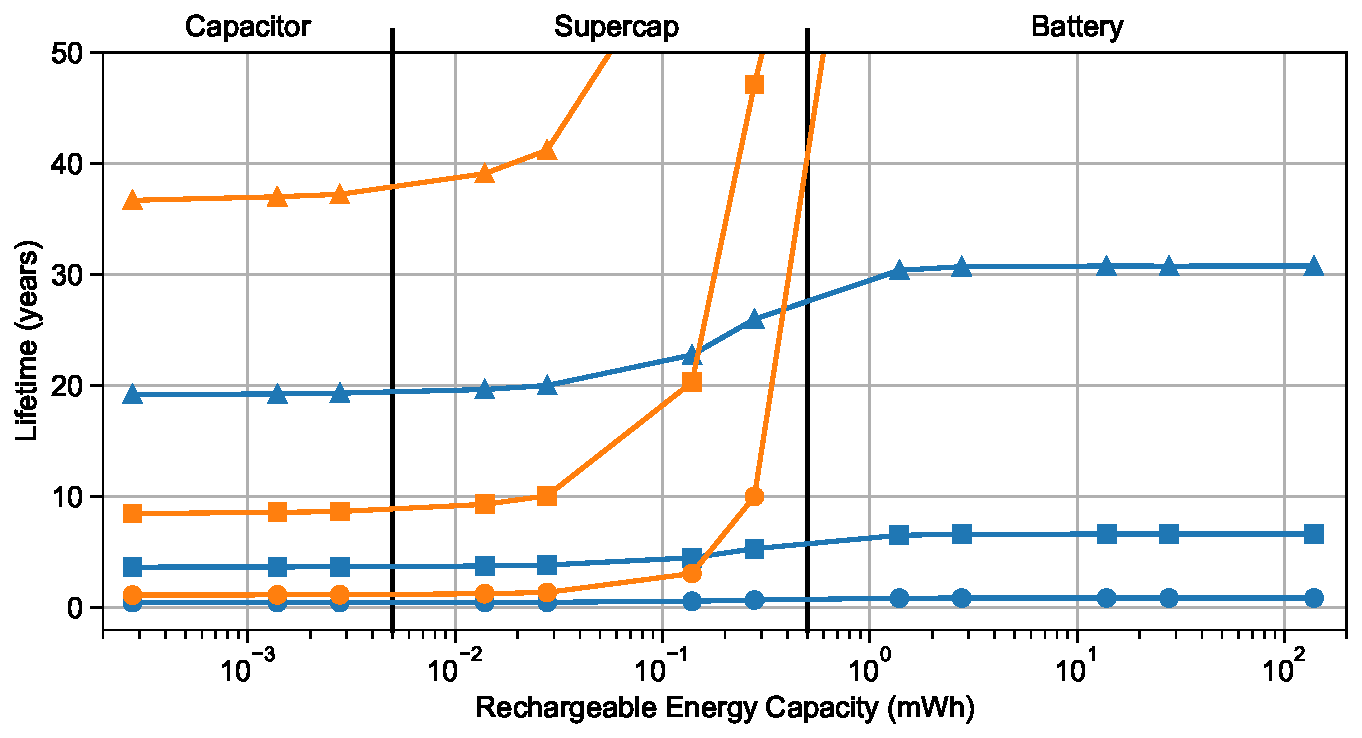
\includegraphics[width=0.85\linewidth]{figs/capacity/primary/door_occu_life_vs_sec_size}
      \caption{Reactive Application}
    \label{fig:primary:eventsec}
  \end{subfigure}
  \caption{
    \normalfont
    Estimated lifetime
    when varying secondary energy capacity for different harvesting scenarios
    and backup energy storage sizes. The periodic application's period
    is 30\,s and the reactive application events are scaled to
    represent a maximum of 2000 events per hour.
    %Harvesting scenarios and workloads
    %are described in \cref{sec:overview} and \cref{tab:capacity:rep}, and
    The backup
    sizes correspond to those found in common coin cell batteries:
    90\,mWh, 720\,mWh, 4500\,mWh for the CR927, CR2032, and CR123A respectively.
    As the ability to capture
    more harvested energy increases, the sensors lifetime increases.
    In some scenarios, expected
    lifetime becomes unbounded as the device is able to subsist entirely on harvested
    energy.
    %All scenarios experience substantial
    %increases in lifetime from increased secondary storage size.
    We see a 2-4x increase in lifetime estimates from the smallest to largest
    capacity simulated, if we only consider bounded results.
    We emphasize that
    these lifetime estimations are
    just estimations, and while we do model the 1\,\%/year leakage
    typical of coin cells, we do not consider the unknown
    physical degradation that would be experienced over decades of use.
    }
\end{definefigure*}

\subsection{Necessary Reliability}
this section will be about achieving .99, .999, and 100\% reliability, assuming sufficient \textit{average} energy. What is the cost in energy capacity?

\section{Reliability Requires Backup}
\label{sec:primary}

Increasing secondary capacity greatly improves
reliability.
%for both periodic and reactive workloads.
However, some environmental
conditions and workloads do not reach 100\% reliability regardless of the size
of the secondary store.
%reactive workloads with large secondary
%capacities, some of the
Some results in \cref{fig:reliability}
appear to achieve perfect reliability, but still miss 0.1-2\% of events.
%with
%diminishing returns for increased secondary capacity.
%Additionally, some workloads
Others achieve well below 100\% reliability, %at the upper extents of storage capacity,
and simply require much more energy
than is harvestable. A backup energy store can increase reliability of a system
to 100\%, at the cost of a finite lifetime.
%In both of these case, further increasing secondary
%capacity does not improve reliability.
%and the desired application cannot rely soly on harvested power.
%and we expect that
%workloads which achieve slightly less than perfect reliability are experiencing
%a combination of brief harvesting droughts and high amounts of temporally local activity
%that push the local average power well above that of the average harvested power.
%While the second case may be solved with a sufficiently large secondary-cell, the
%diminishing returns of increasing secondary size and
%unpredictability of some reactive applications
%makes it difficult to rely solely on harvested power.

\subsection{Reliability Required}
\label{sec:primary:reliability}

We argue that 100\% reliability is a significant improvement over
even low failure rates with respect to reliability
%information
%for many applications
and simplicity due to the lack of intermittency.
%that is a consequence
%of reliability.
Many applications, especially human facing ones,
must be reliable to function, and research shows that unreliability
leads to frustration and %lack of
unwillingness to adopt automated solutions~\cite{brushHome11, edwardsHome01, shehanHome07}.
To use energy harvesting sensors for control or feedback of systems with potential
safety issues, inherent unreliability is intolerable.

Worse, intermittent system failures are difficult to detect %and mitigate
because there is no method for distinguishing between lack of energy
and an actual fault. While scheduled communication of current energy state
may help, this would be difficult for systems that only store enough
energy to perform a single operation such as Flicker~\cite{hesterFlicker17},
Gecko~\cite{yervaGrafting12}, and some configurations of
Capybara~\cite{colinReconfigurable18}.

Finally, it is more difficult
to program intermittent systems because programmers or the underlying
programming model must monitor and adapt to available energy with fine
granularity, both of which are non-trivial tasks.
These systems have little ability to correct for failures
even when they are detected.
%A reliable system has the ability to spend more short-term
%energy to correct for detected failures.

\subsection{Lifetime of a Backup Energy Store}
\label{sec:primary:lifetime}

To achieve 100\% reliability and avoid intermittency,
designs can utilize a backup energy store.
%that is pre-charged at the start of the
%node's life.
In instances where the rechargeable source is depleted, the system
can operate from the backup, masking the effects of variable energy income.
When the backup energy store is depleted, we consider the node's lifetime
to be complete, although it could continue
operating intermittently and with lower reliability. This energy store should
be a primary-cell, as they offer very low self-discharge, long shelf life, and
substantial energy density.
%This pre-charged energy store could be accomplished
%by either a large secondary-cell or a primary-cell, but to avoid increasing
%volume significantly this energy store will almost certainly manifest itself
%as a non-rechargeable battery.

An analysis of the reliable lifetime of a node with both energy
harvesting and a backup energy store is shown in \cref{fig:primary}.
%for
%both periodic and event based workloads.
We choose several backup energy
stores with energy equivalent to those found in several types of common
primary-cells. We see that with energy harvesting and a sufficiently
large secondary energy store, nodes can
achieve 100\% reliable lifetimes that exceed
what we can reasonably predict, especially for harvesting scenarios that
exceed the average power of the application. In these scenarios, 
the inclusion of a backup energy store is critical 
to ensure reliability in uncharacteristically adverse conditions.
Even for conditions with
limited energy availability we still observe significant lifetime improvements
due to energy harvesting.
\placefigure[t]{fig:primary}

\begin{definefigure*}{fig:usage}
  \centering
  \begin{subfigure}{0.49\textwidth}
    \centering
    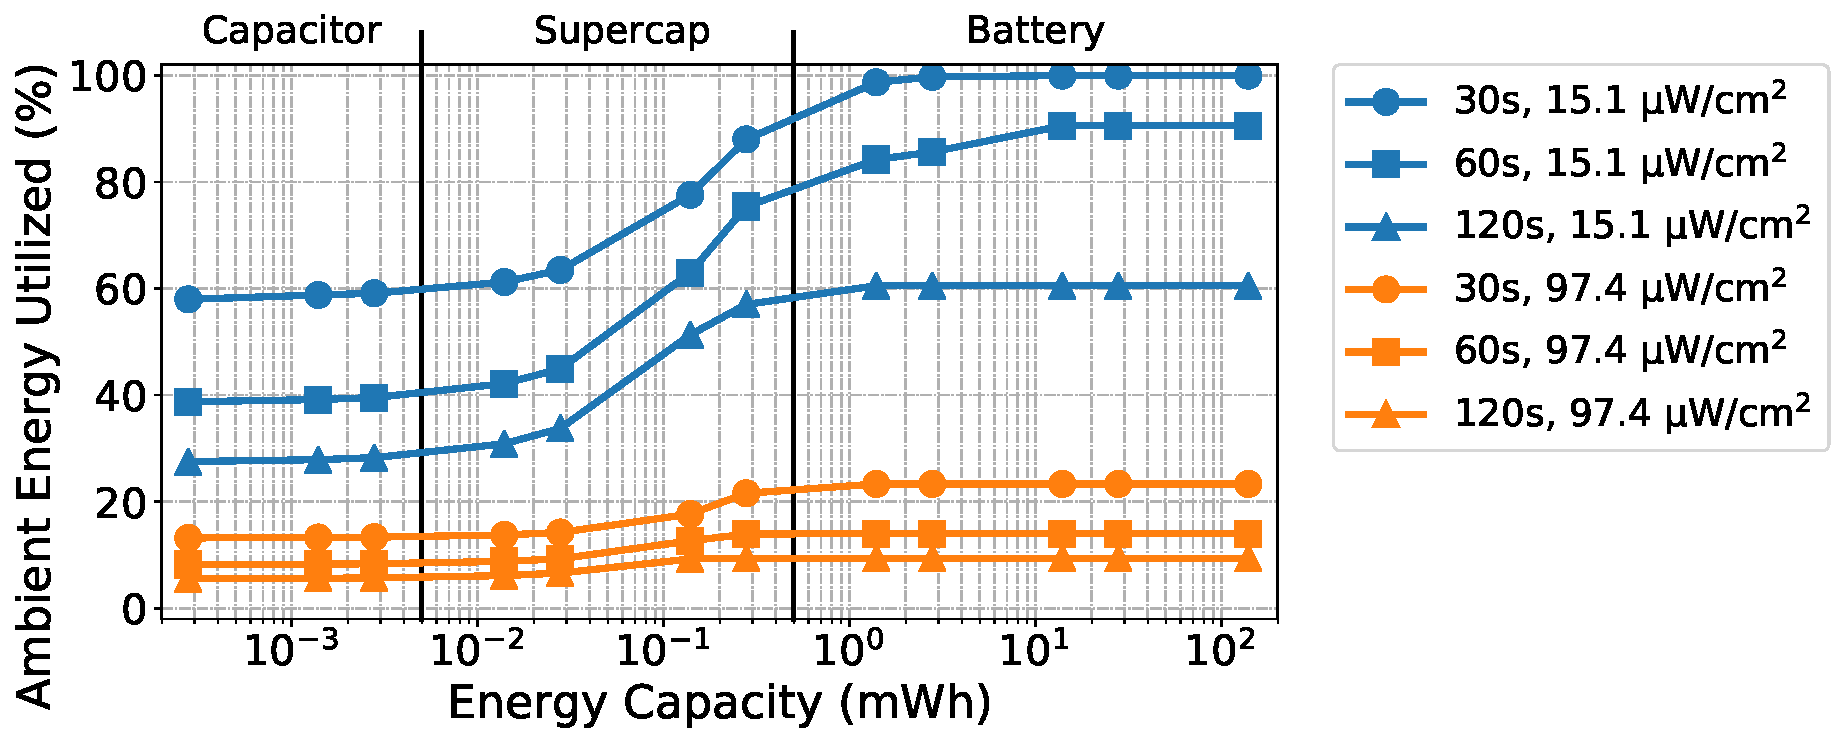
\includegraphics[width=0.9\linewidth]{figs/capacity/sense_and_send/usage_vs_secondary_size}
    \caption{Periodic application}
    \label{fig:usage:sensesec}
  \end{subfigure}
  \begin{subfigure}{0.49\textwidth}
    \centering
    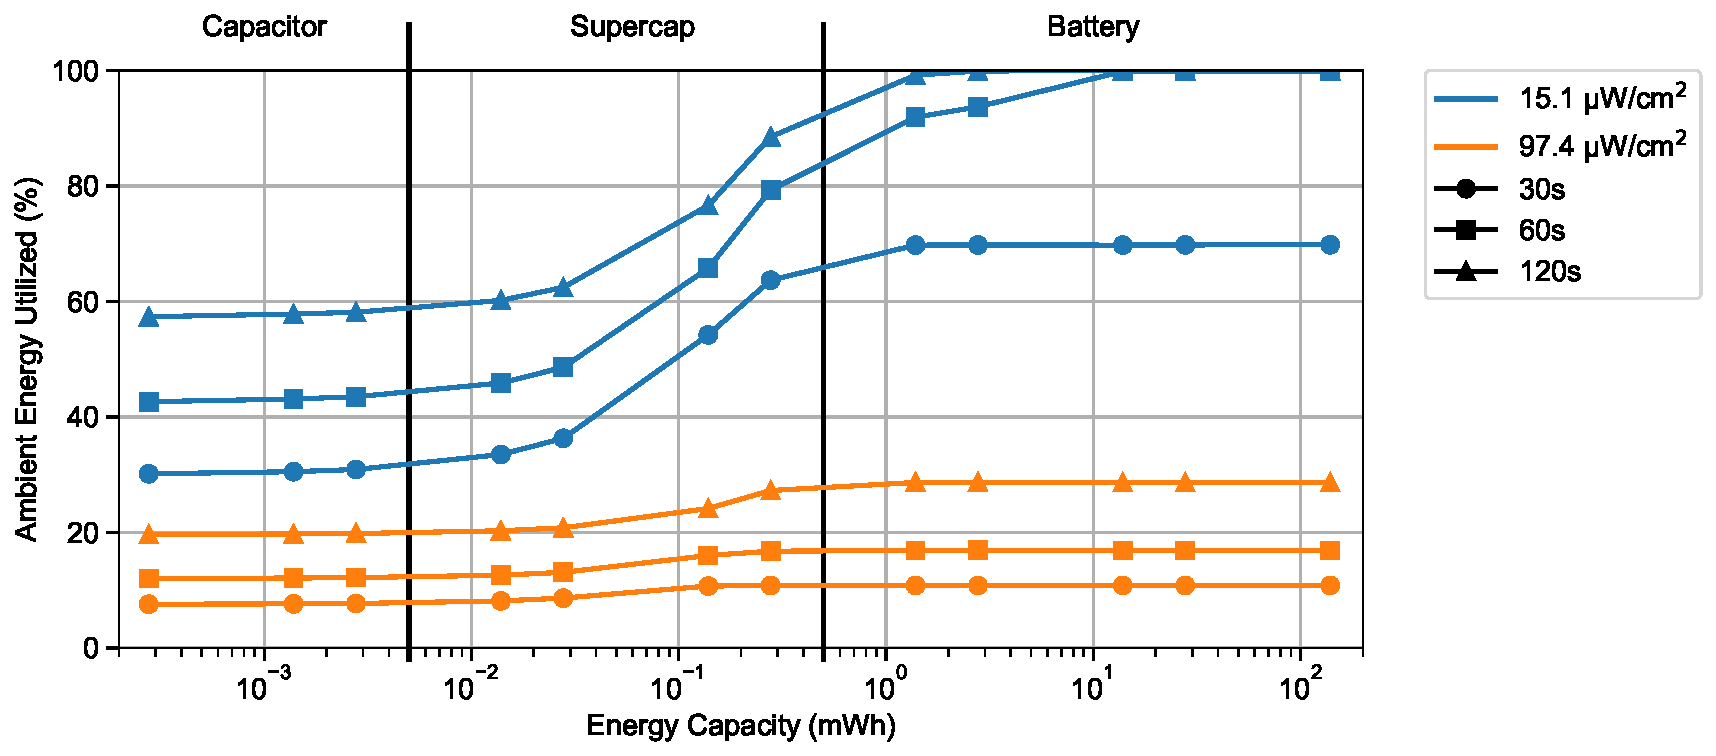
\includegraphics[width=0.9\linewidth]{figs/capacity/door_occupancy/usage_vs_secondary_size}
    \caption{Reactive application}
    \label{fig:usage:eventsec}
  \end{subfigure}
  \caption{\normalfont Ambient energy utilization
    as a function of idealized secondary storage capacity for different
    harvesting scenarios and workloads. The harvesting scenarios and workloads
    are described in \cref{sec:overview} and \cref{tab:capacity:rep}.  The x-axis is
    split by energy capacities possible with capacitors, supercapacitors, and
    batteries. The upper extents of capacity for (super)capacitors represent
    ten 100\,\si{\micro\farad} tantalum capacitors~\cite{tantalumDatasheet}, and one
    large 220\,mF supercapacitor~\cite{murataCap}. Larger capacitors exist, but
    are not appropriate for use on a small sensor node.  As energy storage increases, the harvestable energy used in
    the application also increases, implying
    increased application performance.  Some scenarios, such as the periodic
    30\,s, 15.1\,\uW/cm\textsuperscript{2} case, reach 100\% utilization at
    high secondary capacities indicating that available energy is not
    sufficient to meet the application's requirements.
    Generally, for both workloads and irradiance traces, from
    the smallest to largest capacity simulated, we see a 1.4-2.3x increase in
    utilized energy.
    }
\end{definefigure*}

\begin{definefigure*}{fig:reliability}
  \centering
  \begin{subfigure}{\textwidth}
    \begin{subfigure}{0.5\textwidth}
      \centering
      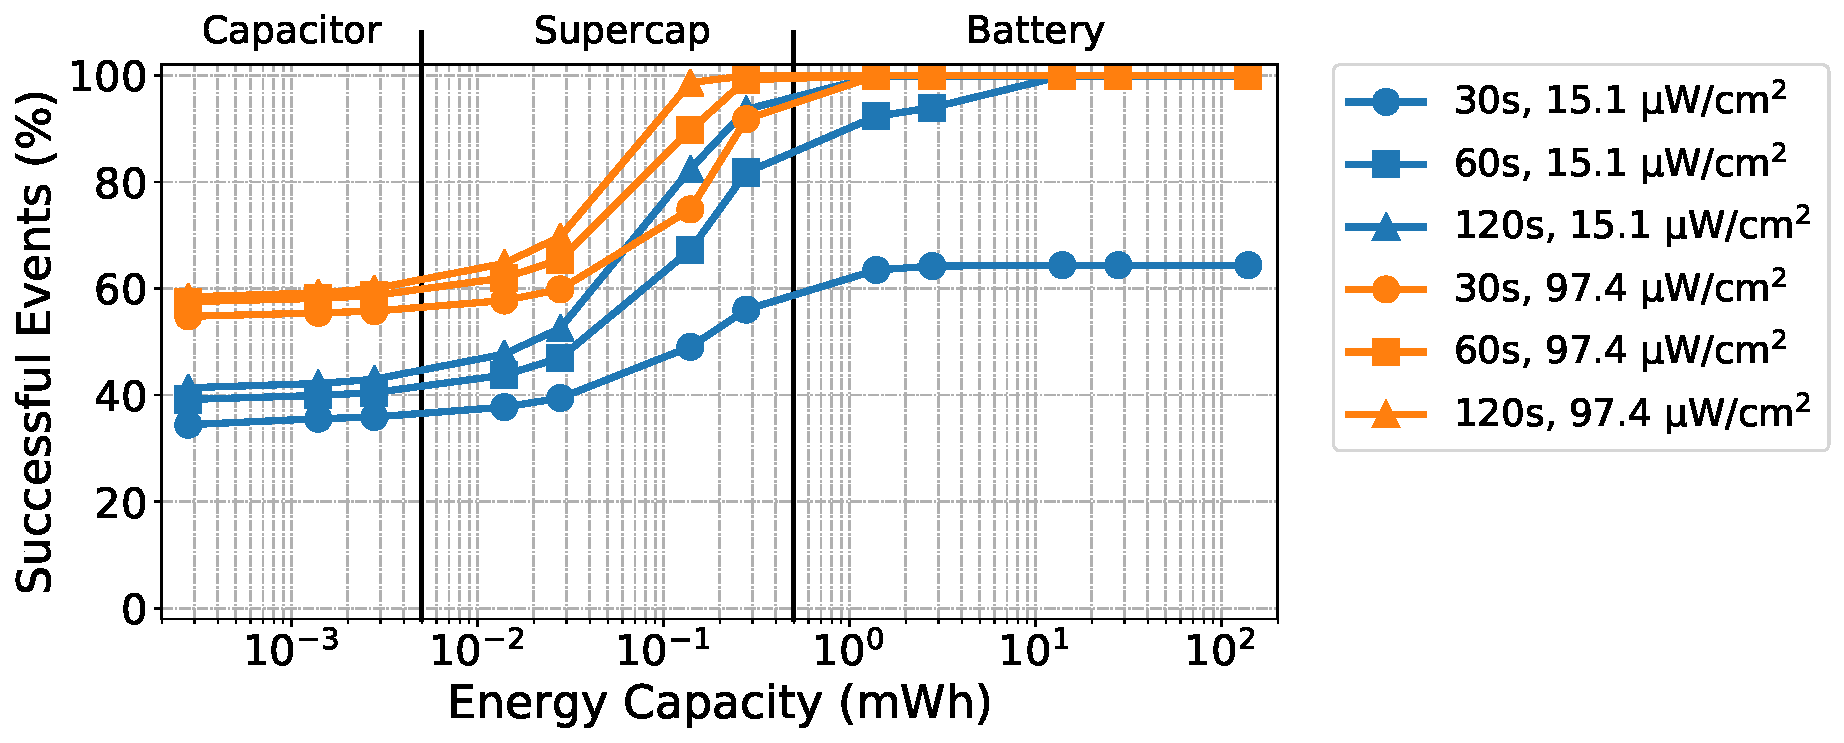
\includegraphics[width=0.9\linewidth]{figs/capacity/sense_and_send/events_vs_secondary_size}
        \caption{Periodic application}
      \label{fig:reliability:sensesec}
    \end{subfigure}
    \begin{subfigure}{0.5\textwidth}
      \centering
      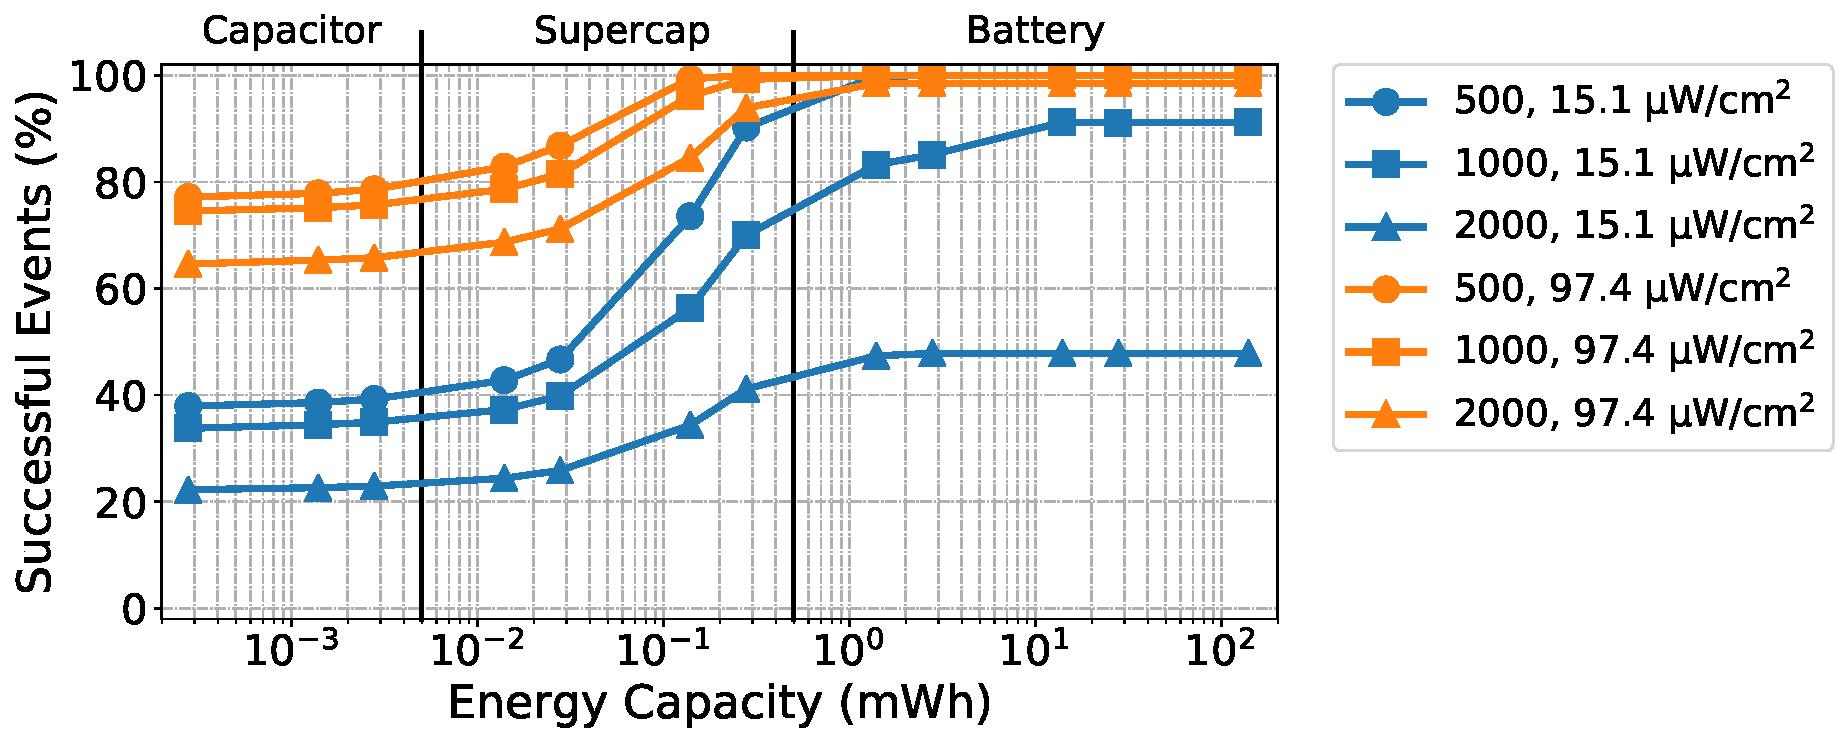
\includegraphics[width=0.9\linewidth]{figs/capacity/door_occupancy/events_vs_secondary_size}
      \caption{Reactive application}
      \label{fig:reliability:eventsec}
    \end{subfigure}
  \end{subfigure}
  \begin{subfigure}{\textwidth}
    \begin{subfigure}{0.5\textwidth}
      \centering
      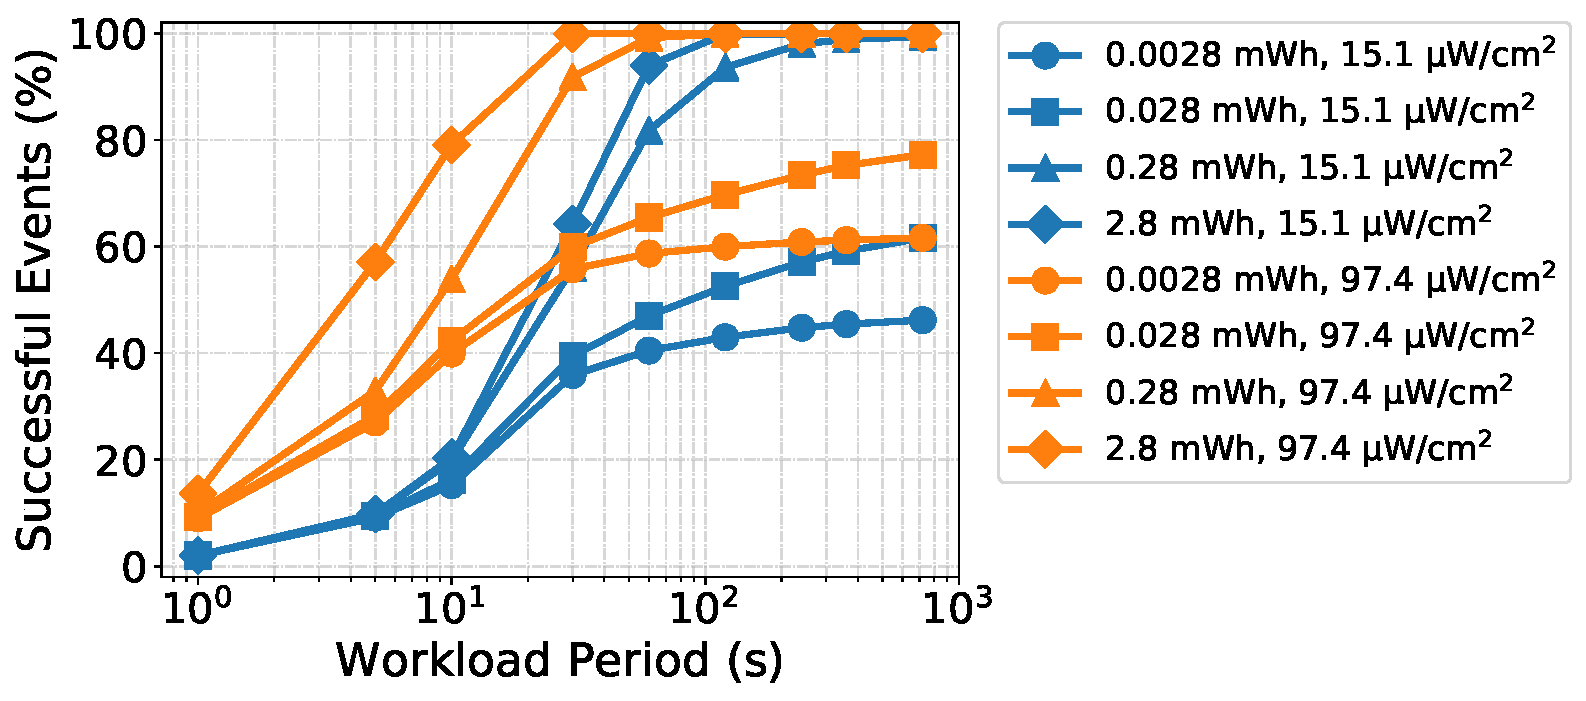
\includegraphics[width=0.9\linewidth]{figs/capacity/sense_and_send/events_vs_period}
      \caption{Periodic\textemdash varying period}
      \label{fig:reliability:senseper}
    \end{subfigure}
    \begin{subfigure}{0.5\textwidth}
      \centering
      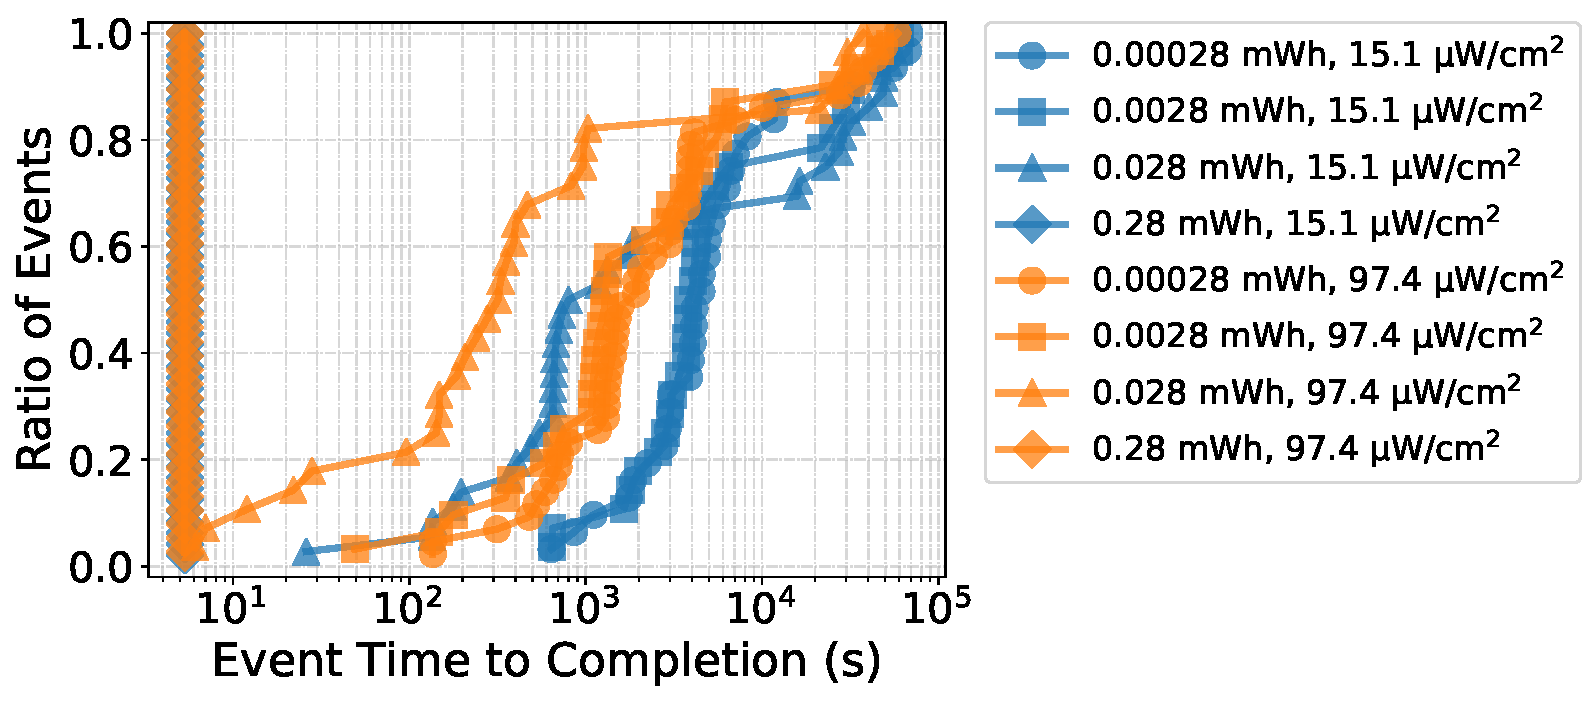
\includegraphics[width=0.9\linewidth]{figs/capacity/ota_update/ttc_ota}
      \caption{Long-running, high energy event}
      \label{fig:reliability:otattc}
    \end{subfigure}
  \end{subfigure}
  \caption{
    \normalfont
    Workload reliability
    for different harvesting scenarios, workloads, and idealized secondary storage sizes.
    We define reliability as the percentage of successfully completed events.
    As expected,
    workload reliability follows the same
    trend as energy utilization, improving with increased secondary energy
    storage. For both periodic and reactive workloads, from the smallest to
    largest capacity simulated, we see a 1.4-2.7x improvement in availability.
    In (c) we investigate the period at which different secondary storage sizes
    meet a specific reliability, showing that even with infrequent periodic
    workloads, small amounts of secondary storage have low reliability while
    larger secondary stores reach near 100\% reliability. (d) shows a CDF of
    time to completion for events in the long-running workload. In this
    workload, events are not atomic, and can be paused and resumed based on
    available energy. With secondary capacities that are large relative to the
    workload (which takes 93\,mJ) we see immediate completion.
    However, performing the event on smaller secondary capacities can take
    between three hours and a day to complete even for scenarios with large
    amounts of harvestable ambient energy.
    }
\end{definefigure*}

\begin{definetable}{tab:capacity:rep}
    \begin{threeparttable}
    \centering
    \begin{subtable}{\columnwidth}
            \begin{tabular}{l | c | c | c | c }
                \thead[l]{\\Irradiance \\Trace} & \thead{\\ \\ Total Days} & \thead{Average\\Power\\(\textmu W/cm\textsuperscript{2})} & \thead{90\textsuperscript{th} Percentile\\Daily Power \\(\textmu W/cm\textsuperscript{2})} & \thead{10\textsuperscript{th} Percentile\\Daily Power \\(\textmu W/cm\textsuperscript{2})} \\\hline
                EnHANTs A   & 394  & 15.1     & 25.0      & 5.2\\
                EnHANTs D   & 311  & 97.4     & 256.5     & 24.8\\
                %Enhants C   & 327  & 745.4    & 1610.0    & 176.1\\
            \end{tabular}
            \caption{Indoor photovoltaic irradiance traces}
            \label{tab:capacity:rep_trace}
        \end{subtable}\\
        \begin{subtable}{\columnwidth}
            \centering
            \begin{tabular}{l | c | c | c}
                Workload Class & Energy per Event (uJ) & Average Period & Average Power (\textmu W)\,\tnote{a}\\\hline
            \multirow{4}{*}{Periodic}   & \multirow{4}{*}{586}  & 10\,s                 &  58.6     \\
                                        &                       & 30\,s                 &  24.5     \\
                                        &                       & 60\,s                 &  14.7     \\
                                        &                       & 120\,s                &  9.8      \\\hline
            \multirow{3}{*}{Reactive}   & \multirow{3}{*}{86}   & 3.4\,s\,\tnote{b}     &  25.3     \\
                                        &                       & 6.8\,s\,\tnote{b}     &  17.6     \\
                                        &                       & 13.6\,s\,\tnote{b}    &  11.3     \\\hline
                 Long-Running           & 93,300                 & 2\,weeks\,\tnote{c}  &  5.1      \\
            \end{tabular}
            \caption{Representative workloads}
            \label{tab:capacity:rep_work}
        \end{subtable}
    \end{threeparttable}
    \small
    \begin{tablenotes}[para]
    \item[a] Average power includes an average 5\,\textmu W idle power, measured in \cref{sec:impl:permamote}.\\
    \item[b] Event times are based on a Poisson distribution for each hour of the day and drawn every second. The distribution is parameterized by collected entryway data then scaled.\\
    \item[c] Event time is based on a uniform distribution and drawn every second.
    \end{tablenotes}
    \caption{\normalfont Representative harvesting conditions and workloads.
    To evaluate different energy harvesting storage techniques, we define a set of energy harvesting
    conditions and workloads that are representative of common sensing applications. We choose two
    real irradiance traces with different magnitudes and distributions of available energy.
    These traces are summarized in \cref{tab:capacity:rep_trace}.
    We define three
    workloads: periodic, reactive, and long-running, and we characterize those workloads
    for different event frequencies. The energy used for each event is measured
    on our reference hardware described in \cref{sec:impl:permamote}.
    Statistics for the three workloads are described in \cref{tab:capacity:rep_work}.
    }
\end{definetable}

\begin{definetable}{tab:parameters}
    \centering
    \begin{adjustbox}{width=\columnwidth}
    \begin{tabular}{lll}
\hline
\textbf{Config Type}& \multicolumn{1}{l}{\textbf{Parameter}}                   & \multicolumn{1}{l}{\textbf{Description}} \\ \hline
\textbf{Device}     & \texttt{operating\_voltage}                              & Output voltage of the power subsystem    \\
                    & \texttt{boost\_efficiency}                               & Efficiency of the boost converter        \\
                    & \texttt{frontend\_efficiency}                            & Efficiency of the harvesting frontend    \\ \hline
\textbf{Secondary}  & \texttt{capacity}                                        & Capacity of secondary in joules or mAh   \\
                    & \texttt{esr}                                             & Equivalent series resistance in ohms     \\
                    & \texttt{leakage\_constant}                               & Factor for capacity dependent leakage    \\
                    & \texttt{\string{max, min\string}\_hyst}                  & Secondary capacity upper/lower hysteresis\\ \hline
\textbf{Primary}    & \texttt{capacity}                                        & Capacity of primary in mAh               \\
                    & \texttt{leakage\_percent}                                & Percent capacity leakage per year        \\ \hline
        \textbf{Harvester}  & \texttt{area}                                    & Area of solar harvester in cm\textsuperscript{2}\\
\textbf{(Solar)}    & \texttt{efficiency}                                      & Efficiency of solar panel                \\ \hline
%\textbf{Workload}   & \texttt{type}                                            & Periodic or Reactive                     \\
%                    & \texttt{period/scale}                                    & Period, or scale for average \# of events \\
%                    & \texttt{opportunistic}                                   & Ignore period, and perform events ASAP   \\
%                    & \texttt{sleep\_current}                                  & Current draw of system in low power mode \\
%                    & \texttt{startup\_\string{energy, period\string}}         & Energy, time required for startup        \\
%                    & \texttt{event\_\string{energy, period\string}}           & Total energy, time required for work event \\
%                    & \texttt{atomic}                                          & Workload is atomic, or intermittent      \\
%                    & \texttt{event\_period\_min}                              & If not atomic, minimum splitable period  \\ \hline

    \end{tabular}
    \end{adjustbox}
    \caption{\normalfont Simulation configuration parameters.
      A representative set of available configuration options for our
      simulation of a sensor with secondary storage and energy harvester, a
      primary-cell, or both. A secondary-cell can be configured with a
      hysteresis, with a lower bound set to \texttt{min\_hyst}
      and an upper bound of \texttt{max\_hyst}.
      %This upper bound must represent
      %the minimum amount of
      %energy to do useful work.
      %Therefore, the upper bound of charging
      %hysteresis is set to \texttt{secondary\_max\_hyst}.
      %Workloads are
      %configured to be either periodic or reactive, and workload intensity is
      %determined by period, or a scaling factor determining the average number
      %of events picked from a random distribution.
      }
\end{definetable}
\begin{definefigure}{fig:capacity:statemachine}
    \centering
    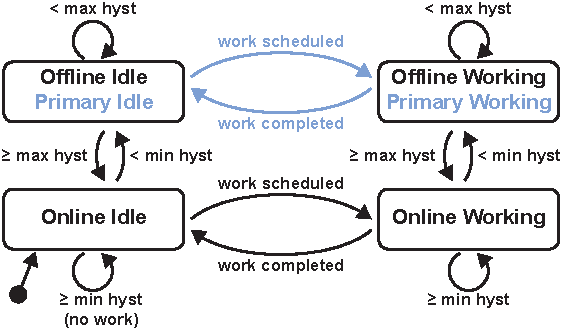
\includegraphics[width=\columnwidth]{figs/capacity/model_state_machine}
    \caption{\normalfont Model state machine.
    A modeled device can be in one of four states: \textsf{Offline Idle},
    \textsf{Online Idle}, \textsf{Online Working}, and \textsf{Offline
    Working}. When a device is \textsf{Offline Idle}, it has run out of energy
    and is off. If a device is \textsf{Online
    Idle}, it is on and in deep sleep, ready to perform work if triggered. If
    triggered, a device moves to \textsf{Online Working}, where it performs a
    portion of a work event.  If a workload is atomic, workload events
    \textit{must} be completed in one \textsf{Online Working} step, without any
    transitions to an offline state.  \textsf{Offline Working} means that while
    working on a non-atomic task, the device ran out of energy, checkpointed,
    and is waiting to harvest more and resume its task.  For devices
    configured with a primary-cell, \textsf{Offline Idle} and \textsf{Offline
    Working} become \textsf{\textcolor{primary-blue}{Primary Idle}} and
    \textsf{\textcolor{primary-blue}{Primary Working}} respectively.  In these
    states, outgoing energy is charged against the primary-cell and the device
    remains online and able to perform work for the life of the primary-cell.
    %State transitions are determined by incoming energy, the state of charge of
    %the secondary storage, and the generated work schedule from workload
    %parameters.
    }
\end{definefigure}

\section{\name Implementation}
\label{sec:impl:permamote}

%We discuss the implementation of both the model used to generate the results
%of \cref{sec:store} and \cref{sec:primary}, and the \name hardware that
%is based on these results. All of our hardware and software will be made
%\textbf{open source} for use by other researchers.


\begin{definetable}{tab:components}
    \begin{threeparttable}
    \centering
    \scriptsize
        \centering
        \scriptsize
        \begin{tabular}{l | l | c | c}
            Component                           &  Function                     & Active Power          & Idle Power \\\hline
            \multirow{2}{*}{Nordic NRF52840}    & Processor                     & 56\,\uA/MHz           & 940\,nA\,\tnote{a}  \\
                                                & Radio                         & 5.2\,mA @ 0\,dbm      & \textemdash\,\tnote{a}\\
            Ambiq AB1815-T3                     & Real time clock               & 55\,nA                & N/A\,\tnote{b}  \\
            ST Micro LIS2DW12                   & Accelerometer                 & 1\,uA @ 12.5\,Hz      & 50\,nA  \\
            Maxim MAX44009                      & Light sensor                  & 650\,nA               & N/A\,\tnote{b}  \\
            Intersil ISL29125                   & Color sensor                  & 56\,\uA               & 500\,nA  \\
            Silicon Labs SI7021                 & Humidty sensor& 1.5\,\uA @ 1\,Hz      & 60\,nA  \\
            TE Connectivity MS5637              & Pressure sensor               & 0.6 - 5\,\uA @ 1\,Hz  & 10\,nA  \\
            Panasonic EKMB11011                 & PIR Occupancy                 & 100\,\uA              & 1\,uA  \\
        \end{tabular}
    \end{threeparttable}
    \begin{tablenotes}[para]
    \scriptsize
    \item[a] Sleep current for both processor and radio.
    \item[b] No shutdown or idle mode.
    \end{tablenotes}
    \caption{
    \normalfont
    The components used in \name.
    These components are among the lowest power options available, and
    are even 2-4x lower power than those used on relatively recent
    systems such as BLEES, Flicker, Capybara, and Hamilton.
    }
    %Technology
    %scaling for embedded sensors, processors, and radios
    %has driven down the average power of a sensor node much closer to the
    %harvestable solar energy available in indoor lighting conditions. This allows
    %more systems to subsist or achieve extended lifetimes through energy harvesting.
\end{definetable}

\begin{definefigure}{fig:permamote}
    \centering
    \begin{subfigure}{0.7\columnwidth}
        \centering
        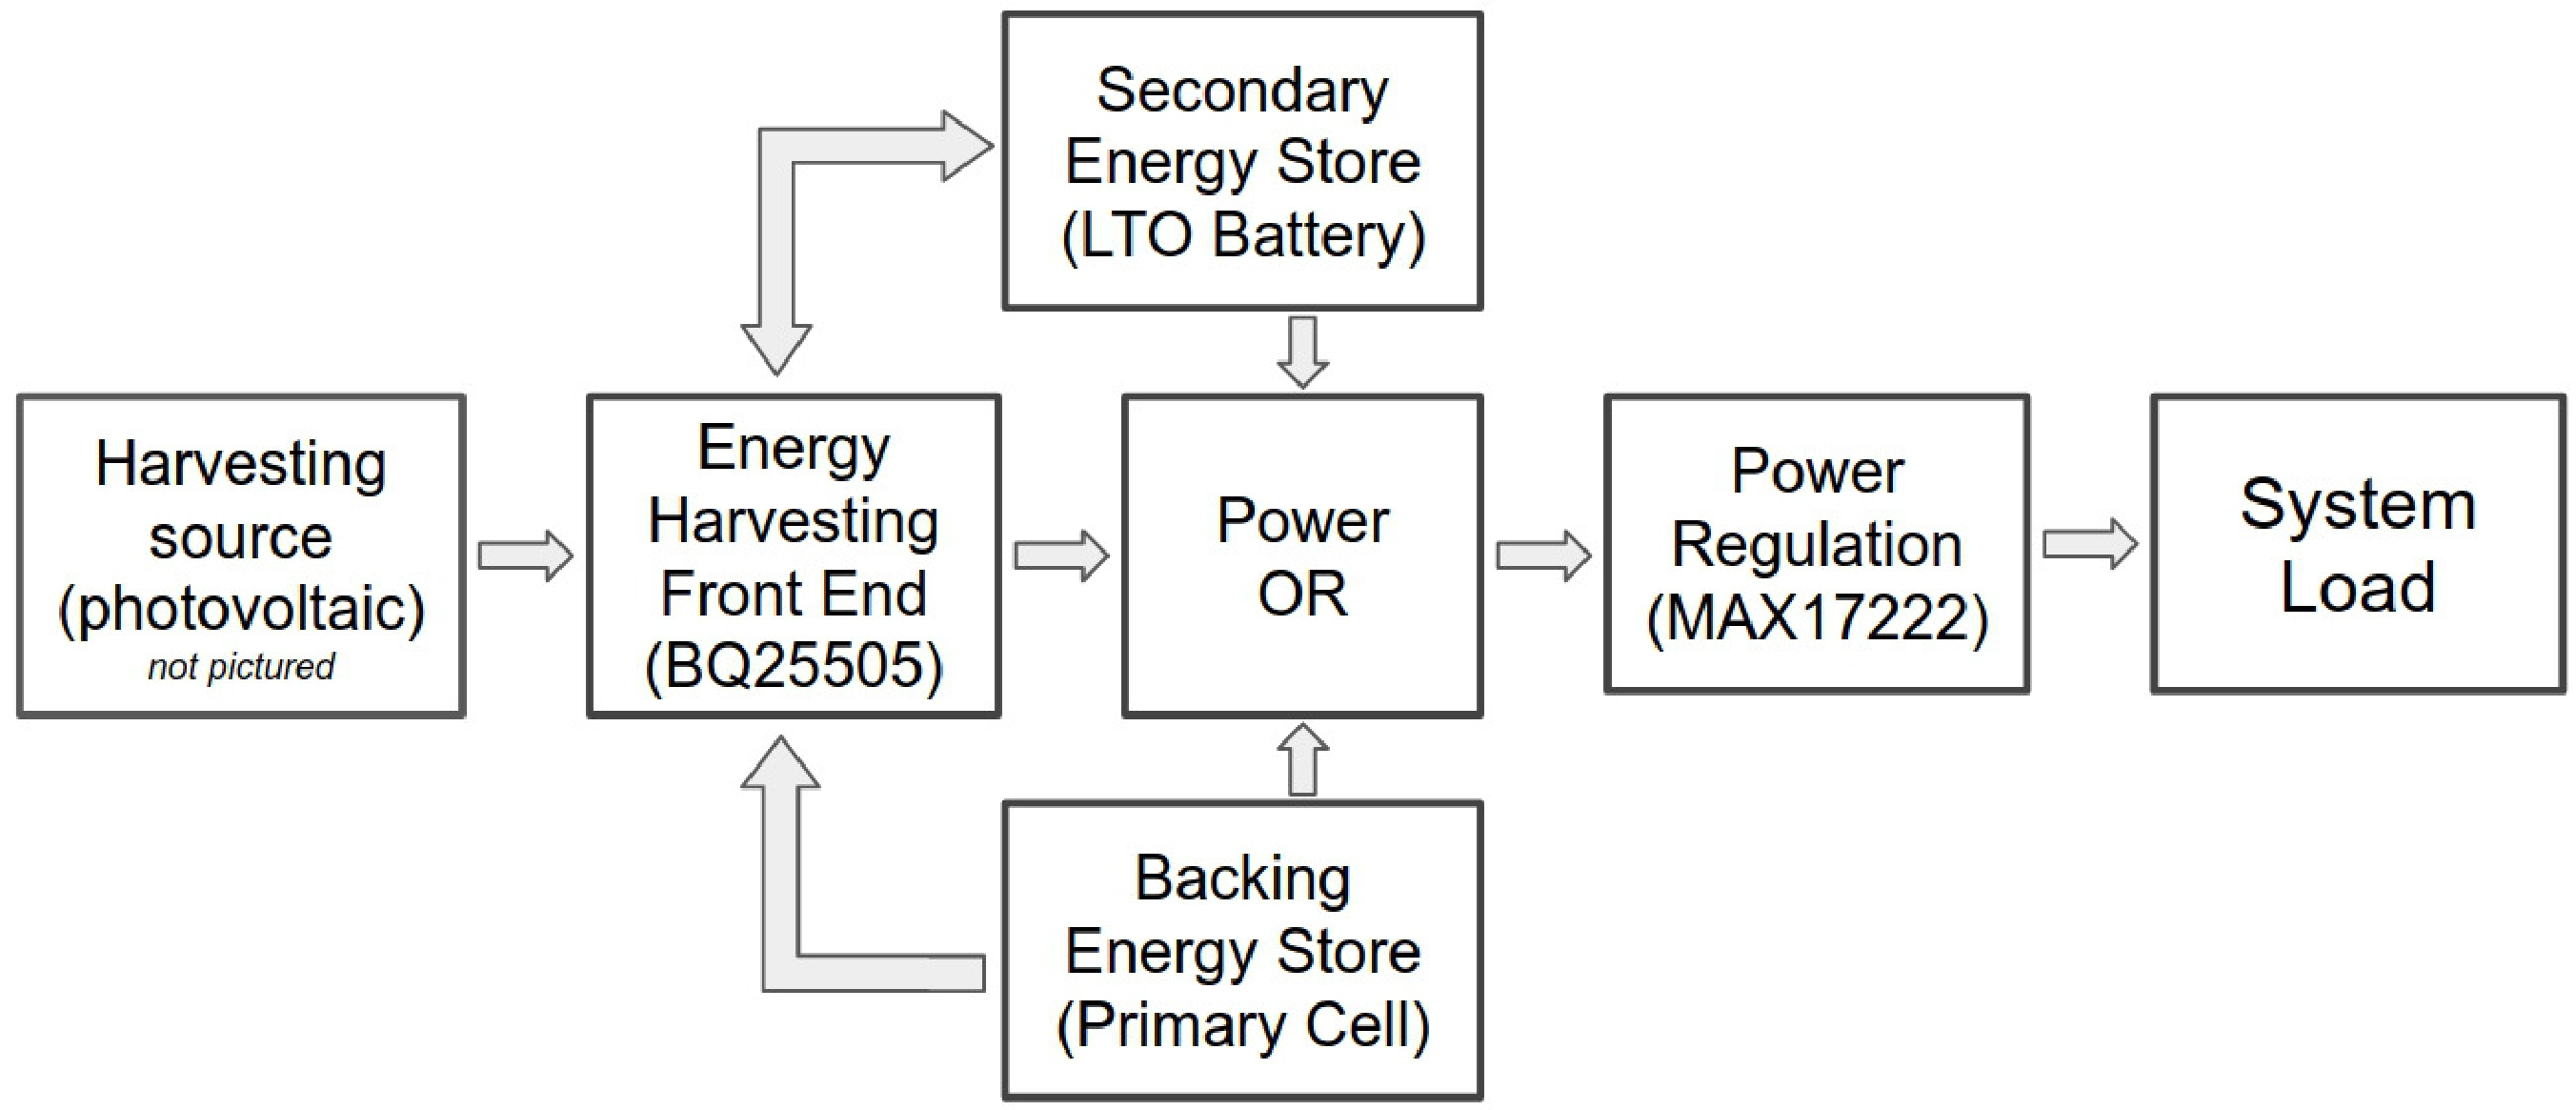
\includegraphics[width=\textwidth]{figs/capacity/arch}
        \caption{Harvesting and storage architecture}
    \end{subfigure}
    \begin{subfigure}{0.29\columnwidth}
        \centering
        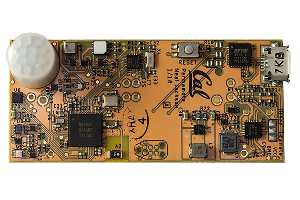
\includegraphics[width=\textwidth,angle=90]{figs/capacity/permamote}
        \caption{Hardware}
    \end{subfigure}
    \caption{\normalfont The \name power supply architecture is informed by the
    findings in \cref{sec:store,sec:primary}. An
    LTO battery is recharged by a solar panel. When the battery is depleted,
    a primary-cell powers the system, providing reliability and avoiding
    intermittency.
    }
    %We believe this platform will run for 6-36 years for common
    %sensing tasks and indoor lighting conditions before the death of
    %the primary-cell. Even after the primary-cell expires,
    %the sensor node could continue to run intermittently on harvested energy.
\end{definefigure}

We implement the design principals discussed in \cref{sec:store,sec:primary}
in a new sensor called \name. The \name sensing platform
integrates a processor, BLE/802.15.4 radio, and various environmental, lighting,
and occupancy sensors. A picture
and system diagram of \name is shown in \cref{fig:permamote}. All hardware
and software for the platform is open source\footnote{\url{https://github.com/lab11/permamote/tree/master/hardware/permamote}}.\\

\vspace{-6pt}
\noindent
\textbf{Energy Harvesting and Storage.}
\name is powered by an energy harvesting front end that realizes the benefits
of using batteries. It uses the TI BQ25505 energy harvesting IC, which
harvests energy while monitoring both
rechargeable and backup energy stores,
switching between them at user-configurable voltages~\cite{bq25505}. A
20\,mAh (48\,mWh) LTO battery is charged by an 10.9\,cm\textsuperscript{2} amorphous
silicon solar panel~\cite{LTODatasheet, LTODatasheet2}. We limit the apparent
capacity of this battery to ensure
longer cycle lifetime as described in \cref{sec:battery}, but still have 24\,mWh of
energy storage, more than the capacity required to achieve the reliability and energy utilization
improvements described in \cref{sec:store}. For the backup energy
store, \name uses lithium primary-cells which can be configured to either one or two CR2032 coin
cells or a CR123A cell.
%Primary-cells provide 3-13x more density and 2-12x less
%leakage than a secondary-cell.
%making them more desirable than a single,
%large, pre-charged secondary-cell as the backup store~\cite{LTODatasheet,primary2032, primarycr123a}.
The output of the active battery
is boosted by a MAX17222 regulator, which features high conversion efficiency
(>90\%) at low output currents and operates down to 400\,mV~\cite{max17222}.\\
%We have the ability to monitor harvesting and system currents using
%the iCount method by sensing the voltage of
%the inductor used by the BQ25505 and MAX17222~\cite{duttaEnergy08}. The processor
%is also capable of gating all sensors from the main power supply to save
%power.\\

\vspace{-6pt}
\noindent
\textbf{Processor, Radio and Sensor Selection.}
In designing \name, we search for the newest and lowest power components.
%We feel that it may
To benefit other
platform builders, we document our component selections
along with their key performance metrics. A summary of these
components can be found in \cref{tab:components}.

We note our choice of the Nordic NRF52840 MCU over the more commonly used MSP430FR series
because of its higher efficiency in active mode while offering comparable sleep currents.
Specifically, it only draws 56\,\uA/MHz compared to over 100\,uA/MHz
for the MSP430. Unlike intermittent systems,
we do not rely on the FRAM present on the MSP430FR series chips. While
slightly more efficient
processors and radios exist than those found in the NRF52840,
we value the simplicity of an SoC-based design. \\

\vspace{-6pt}
\noindent
\textbf{Energy Benchmarks}.
The data presented in \cref{tab:components} are benchmarks taken
on the \name platform. We find that a BLE advertisement at 0\,dbm consumes
86\,\uJ and that sampling both light and color sensors and transmitting
them in a BLE advertisement consumes 586\,\uJ. Additionally, the entire system, including
the energy harvesting front end, consumes only 5.0\,\uW in deep sleep with RAM
retained and all sensors powered off. We use the energy numbers from \name as a basis
for our workloads to fairly compare against prior energy storage architectures.
%\subsection{Numerical Model}
%\label{impl:model}
%
%We develop a numerical model that simulates the behavior of energy harvesting
%systems in indoor environments. For this work, we've primarily focused on solar
%energy input, and have tailored the model to use solar energy traces. As
%mentioned, we use the Columbia EnHANTs irradiance traces
%\cite{margolies2015energy}. We process the traces, filling the few periods of
%missing data by copying from a week prior.
%
%The model operates at second granularity, and at each
%step, the amount of incoming energy is calculated based on the input irradiance
%and solar panel configuration. If the device has enough energy to turn on
%and perform the task from the specified workload it does so. If there is
%energy to spare after the task, the device will enter a low power sleep state.
%The model tallies the amount of successful and unsuccessful events that it
%was expected to complete, as well as the percentage of energy used out
%the energy that was available from the harvesting source. To estimate
%lifetime, the model attempts tasks for the totality of solar irradiance
%data present, then extrapolates primary-cell discharge to find its lifetime
%at empty. The one second granularity imposes some limitations, however
%we find that sensor node workloads are rarely more intensive.
%
%If the secondary store is not at capacity
%this incoming energy is stored
%
%If the device is online, it attempts to turn on
%if it has enough energy to do so, otherwise it remains offline and continues to
%fail performing its workload.  If the device is on, it perform tasks from its
%workload. It prioritizes using the energy from its rechargeable store, and if
%depleted, will either go offline or use energy from its primary-cell, if
%available. If it has energy to spare, it enters a low power sleep state. The
%model tallies the amount of successful and unsuccessful events that it was
%expected to complete, as well as the percentage of energy it used out of how
%much was available from the irradiance source. It also performs a linear fit on
%the primary state of charge to estimate lifetime, if applicable to the
%simulated device's configuration.
%
%This
%granularity also limits that of workloads to a second, but we argue
%that realistic sensor workloads are rarely more intensive \hl{cite}.


\placefigure[t]{fig:permamote}


\section{Model Evaluation}
\label{sec:eval}
To evaluate the model, we perform a three-month-long deployment in a partially sunlit room
using i) a primary-cell only system, ii) an intermittent, capacitor-only system, and iii) \name, our
system that features both a secondary and primary-cell. We model these
systems over the same period and compare the availability of \name to the
intermittent system.

\subsection{Model Analysis}
\label{sec:eval:model}
We analyze the deployment of these systems
%in a partially sunlit room for three months
and compare their behavior to our
model's predictions: i) ten CR2032 primary-cell only devices, ii) an
intermittent system configured with just 500\textmu F of capacitance (about
0.36\,\textmu Wh at 2.2\,V), and iii) \name, configured with a 20\,mAh
(48\,mWh) secondary-cell, half of which is usable, and a CR2032 backup.  The
primary-cell only device performs environmental sensing over BLE every second.
The intermittent system  sends a beacon as soon as its capacitor bank is full.
When its energy is depleted, it powers off and charges
again. \name is running the ``sense and send'' workload that we described in
\cref{sec:overview}, and sends illuminance measurements every second. This
workload stresses the model and requires more charge and discharge cycles.  We
use \name illuminance readings to estimate irradiance using the same scaling factors used by
Yerva et al.~\cite{yervaGrafting12}, and use these traces as
model input.\\

\vspace{-6pt}
\noindent
\textbf{Primary-Cell Only.}
We model the workload of the primary-cell system and produce estimates for
lifetime.  Our model predicts the platform lifetime
to be 58 days.  We find that the average lifetime of the 10 devices is 61 days.
%,
%from initial deployment to energy depletion, is 61 days.
\\

\vspace{-6pt}
\noindent
\textbf{Intermittent.}
We model the number of packets sent each hour by the
intermittent system over a three week period, and compare against the results of an actual device in
\cref{fig:eval:pkt}.
The average daily error of the model versus our results is 15\%, with a standard deviation of
17\%. This error can attributed to two primary sources. Illuminance is measured
close to, but not exactly at the solar panel of the test device. Occasional
direct sunbeams, like that experienced on day 16, can illuminate the solar
panel but not the sensor, or vice versa. This
results in a substantial over or underestimate of available light. In addition
to inaccurate light measurements, we introduce error through our estimation of
irradiance. We measure illuminance
instead of irradiance, and must resort to a piecewise linear estimation, when
in reality the relationship is not well defined and non-linear when considering
different light sources. In the case of our estimation, results
indicate that the model consistently underestimates high irradiance measurements.\\
\placefigure{tab:components}
\placefigure[t]{fig:evalcmp}

\vspace{-6pt}
\noindent
\textbf{Secondary and Primary-Cell.}
We compare our model's predicted state of charge to a deployed \name over a seven
day period in \cref{fig:eval:soc}. We estimate state of charge from the reported secondary-cell
voltage,
%,
%and measured voltage
%curves of the installed 20\,mAh battery
and irradiance from
lux measurements. In this figure, the state of
charge cycles between configured battery hysteresis limits, as the workload is
too intense to be sustained by energy harvesting alone.
%and the Permamote must
%use energy from its primary cell.
Flat and upward slopes of the curve represent the
device in hysteresis, using the primary battery to perform its workload. Upper slopes
indicate the secondary cell is charging from harvested energy.
Downward slopes indicate the device is out of hysteresis and is using harvested
energy stored in its secondary battery to perform its workload.
%The device is
%charging and in
%hysteresis during upward
%slopes.
The shaded ``nighttime'' regions are not uniform, as the
deployment environment is occupied by graduate students that occasionally work
late hours or forget to turn off the lights.  The model correctly predicts the
cycling
behavior of the deployed device for two days, but deviates
during the third day. The model predicts that the device would charge above the upper
hysteresis limit and begin supplying energy from the secondary-cell before the
test device actually does.  This inaccuracy, like that of the last of
experiment, is partially due to our inexact estimation of irradiance.  In
addition, real device hysteresis limits are set using resistor networks.  The
resistors used have 1-5\% tolerance, and are susceptible to temperature
changes, which introduces dynamic errors that is not accounted for in our model.
Even though the predicted state of charge deviates after two days, the length
and frequency of periods in which harvested energy is stored and used %in the secondary-cell
are identical to our experimental measurements.
%While our model correctly predicts cycling timing and frequency, it appears the
%state of charge  does not quite match that of the measurements.  This is
%because the voltage measured is not the open circuit voltage, and is affected
%by voltage droop due to the applied system load as well as inflated charging
%voltage from the energy harvesting front end.  Ignoring these effects, the
%cycling of the model's prediction is closely synchronized with the estimated
%state of charge.
%We compare the model's predicted
%state of charge over time to the outputs of systems we
%have deployed. For energy harvesting systems we collect lux measurements
%throughout the deployment and convert lux to irradiance based on the
%data collected in Yerva et al.~\cite{yervaGrafting12}. \\
%\vspace{-6pt}
%\noindent
%\textbf{Permamote.}\\
\subsection{\name Performance}
\placefigure[t]{fig:eval}
\label{sec:eval:permamote}
%In addition to evaluating our model,
We also compare the performance of the
deployed intermittent system and \name. In \cref{fig:evalcmp}, we show the
number of packets sent per hour for two days. \name sends data every
second, while the intermittent system sends as fast as possible. \name is
able to collect and send its data continuously, while the
intermittent system is limited to sending only during the day. This
demonstrates the increased availability afforded by increasing secondary
capacity and including a backup energy store.

We also use our model to explore the estimated performance of \name
compared to prior systems.
To isolate the analysis to just power supply types and sizing, we assume each
system uses the same low-power hardware and is performing the same workload.
The results of this modeling are shown in \cref{tab:related}. Our model estimates that
\name can expect several decades of 100\% reliable lifetime when configured as
it was deployed for this evaluation, albeit configured with a less intense workload.
%While the workload used with \name is not
%sustainable for the multi-decade lifetimes we are targeting, it still
%exemplifies the increase in reliability afforded by including a primary-cell.


\begin{definefigure}{fig:eval}
  \centering
  \begin{subfigure}{\columnwidth}
    \centering
    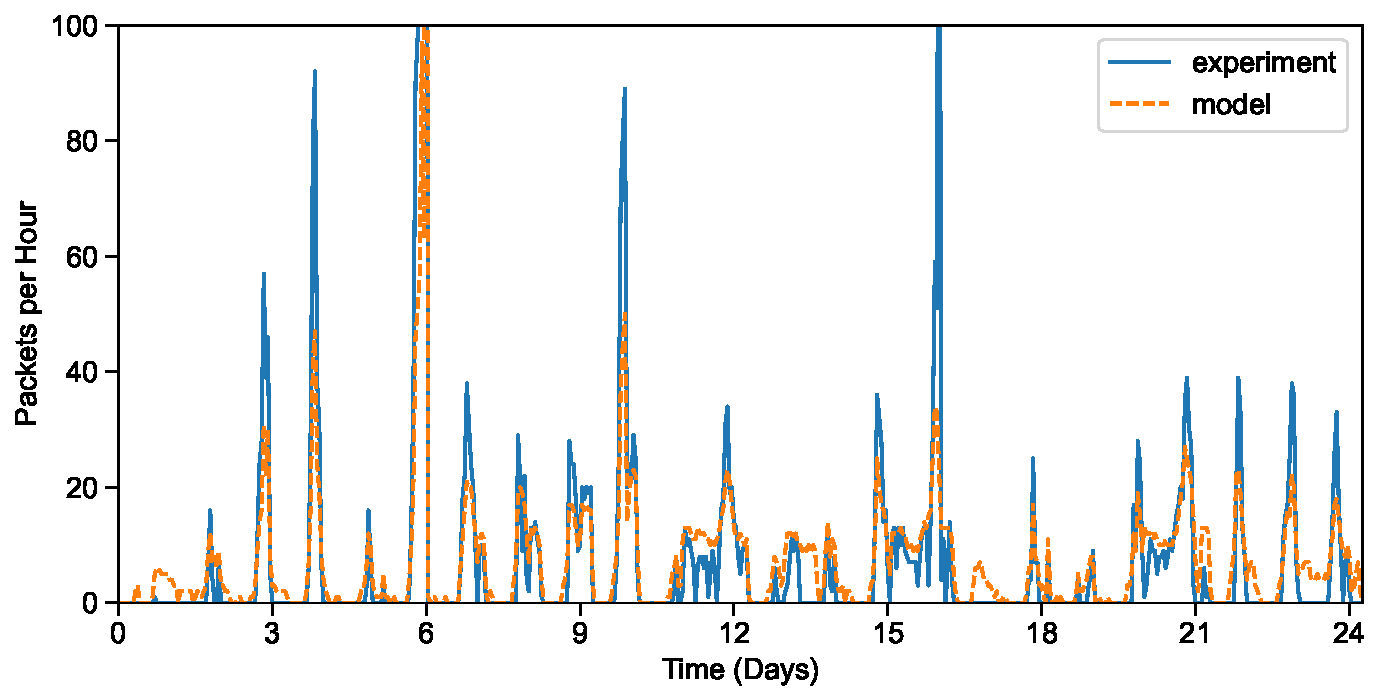
\includegraphics[width=\linewidth]{figs/capacity/experiment_pkt/exp_vs_sim_pkt}
    \caption{Intermittent Node}
    \label{fig:eval:pkt}
  \end{subfigure}\\%\hspace{0.5cm}
  \begin{subfigure}{\columnwidth}
    \centering
    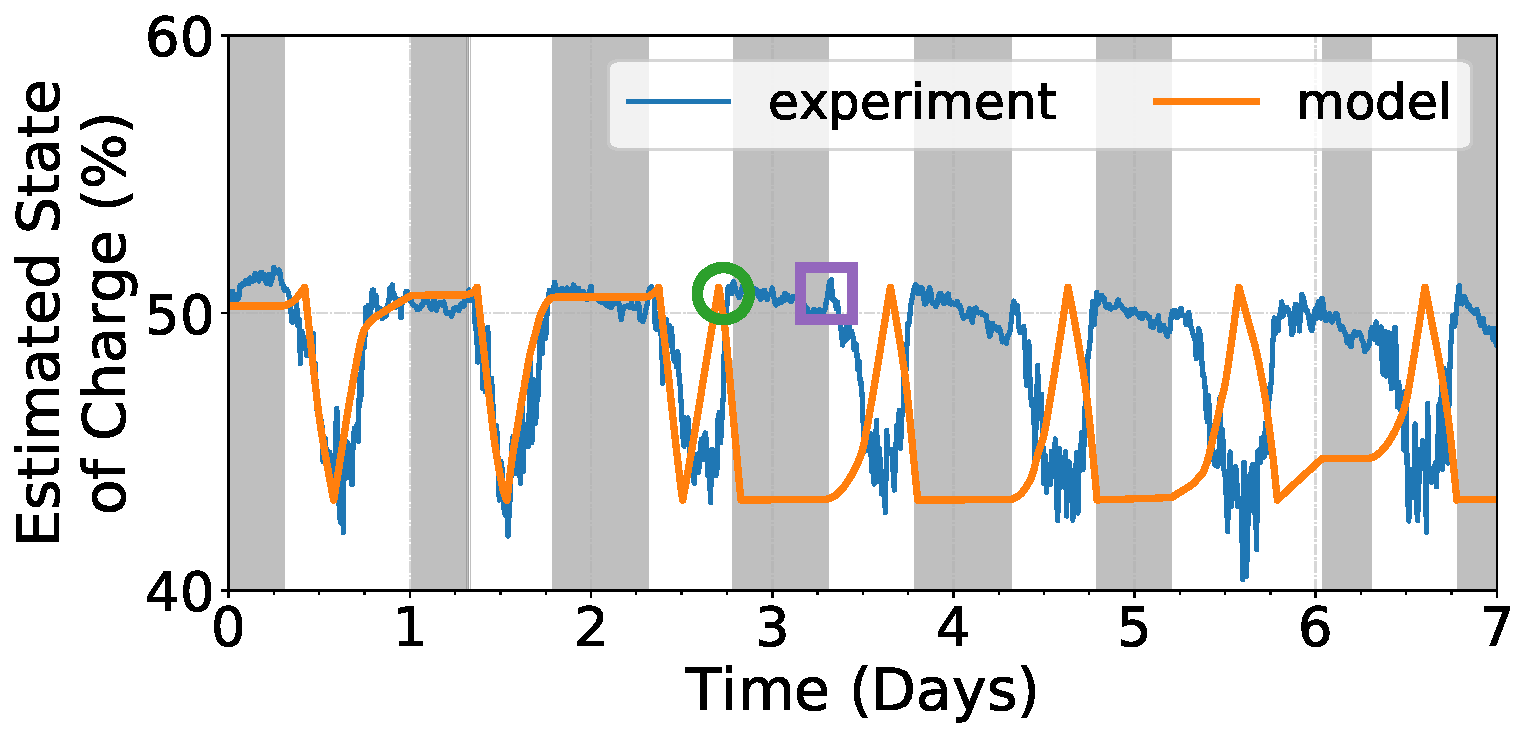
\includegraphics[width=\linewidth]{figs/capacity/experiment_soc/exp_vs_sim_soc}
    \caption{Permamote}
    \label{fig:eval:soc}
  \end{subfigure}
    \caption{Model comparison to deployed hardware.
    \normalfont
    Data from a three month deployment of two systems is used to verify our model.
    (a) We use three weeks of lux measurements %from a month-long deployment
    to estimate irradiance and model the number of packets transmitted by an
    intermittent node. Average daily error is 15\%, with a standard deviation
    of 17\%. (b) We model and measure a \name's state of charge while running a
    ``sense and send'' workload with a 1\,s period for a week, beginning at
    midnight on the first day. Secondary charging hysteresis
    limits of the devices are set at 51\% and 43\%. Shaded regions
    represent periods of low harvestable potential
    (<\,15\,\textmu W/cm\textsuperscript{2}),
    i.e. nighttime. For the first two days, model predictions
    closely track the experimental measurements. Errors
    in hysteresis and irradiance estimation cause the model to reach its upper
    hysteresis sooner than the experiment does, annotated by the
    \textbf{\textcolor{fig-green}{green circle}}. In actuality, the device
    exits charging hysteresis at the peak marked with the
    \textbf{\textcolor{fig-purple}{purple square}}.
    More importantly, the
    frequency and length of periods spent using harvested
    energy collected in the secondary-cell (downward slopes) are identical.
    %For the intermittent node we see our model
    %underestimate the number of transmitted packets by 10-20\% except for the
    %first day which predicts significantly more packets.  We believe this error
    %is primarily due to a piecewise linear estimation of irradiance from our
    %collected illuminance data, when in reality the relationship is complex and
    %non-linear.  For (b) we estimate the state of charge of \name
    %based on the secondary
    %cell voltage. Differences between the estimated state of charge and the
    %modeled state of charge are primarily due to inflated voltage during
    %charging and voltage droop and bounce back when \name
    %draws current from the secondary-cell.
    %Even though estimated state of
    %charge is not accurate due to this voltage swing, it is clear that the
    %timing of charge and discharge aligns between the model and the
    %experimental data.
    }
\end{definefigure}

\begin{definefigure}{fig:evalcmp}
    \centering
    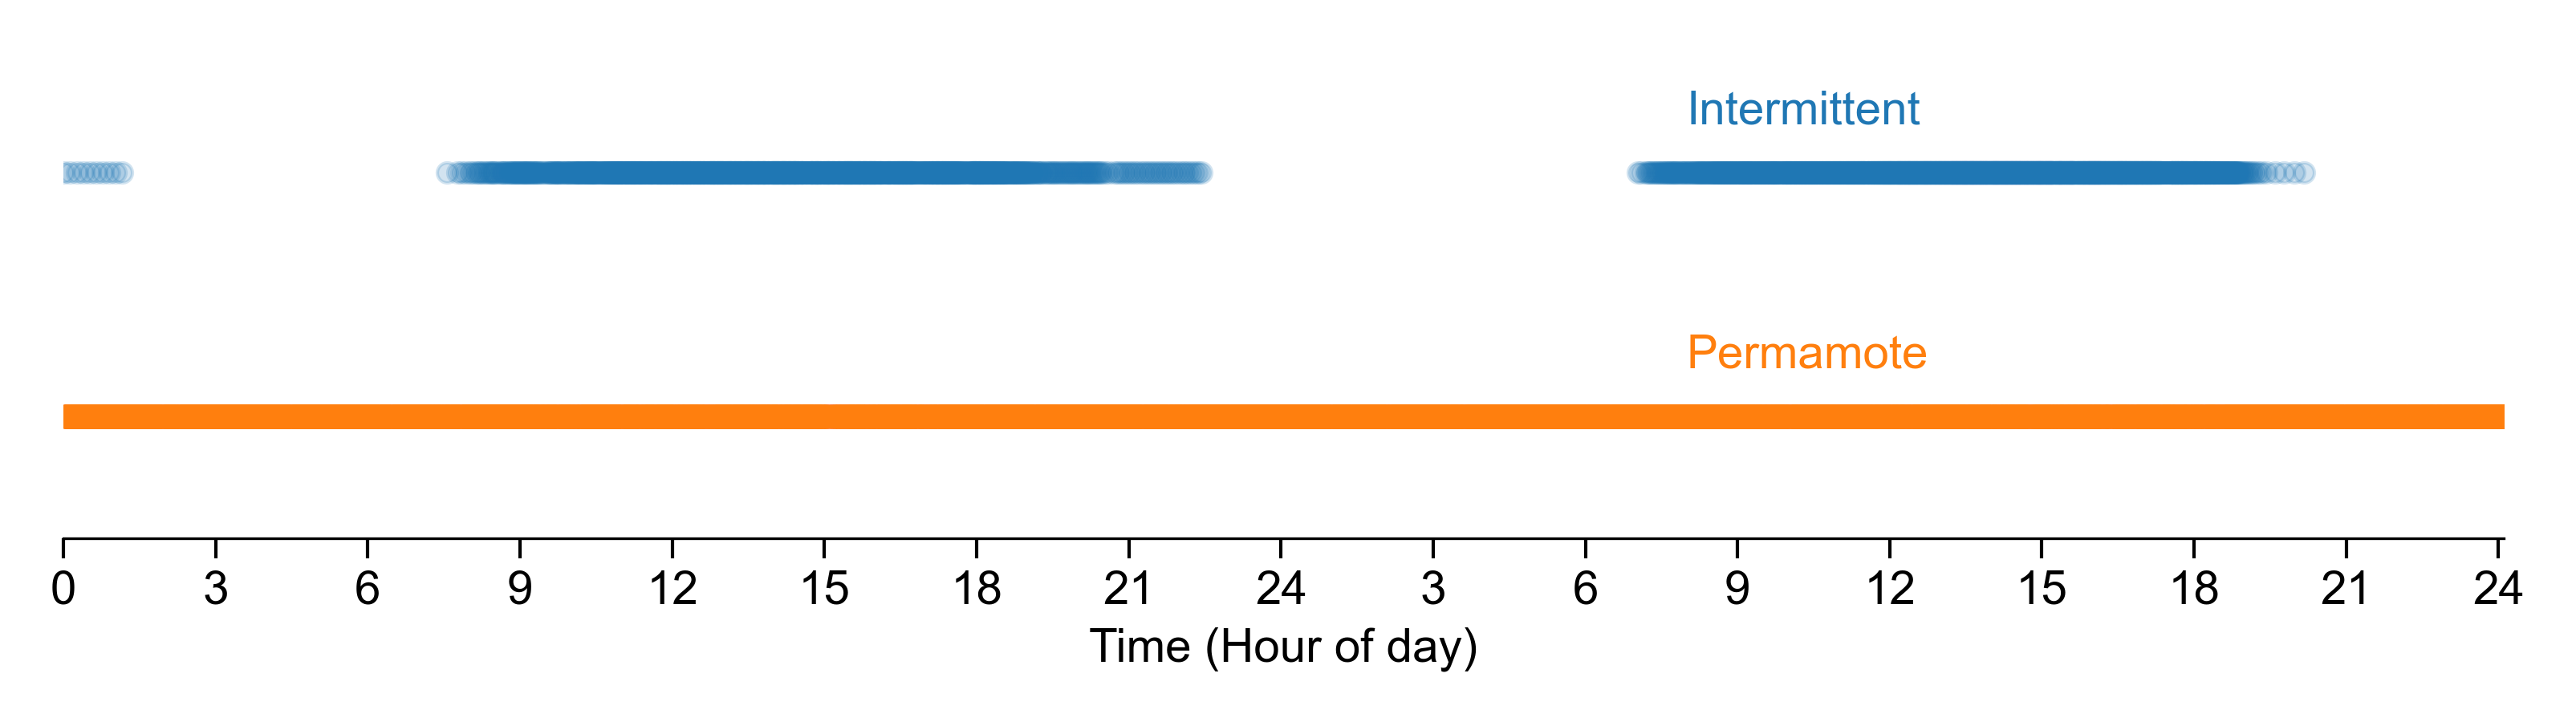
\includegraphics[width=\linewidth]{figs/capacity/experiment_sys_compare/exp_packets_recv}
    \caption{
      \normalfont
        Packets received over two days.
      This figure compares the reliability of an
      intermittent design and \name. \name sends a packet every second and does
      so without fail, while the intermittent system is only able to send when
      light is available.
      %This results in periods at night where the
      %intermittent device does not harvest enough energy to sustain operation.
      }
\end{definefigure}
\placefigure{tab:related}


\section{Summary}
